%
%   This program is free software: you can redistribute it and/or modify
%   it under the terms of the GNU General Public License as published by
%   the Free Software Foundation, either version 3 of the License, or
%   (at your option) any later version.
%
%   This program is distributed in the hope that it will be useful,
%   but WITHOUT ANY WARRANTY; without even the implied warranty of
%   MERCHANTABILITY or FITNESS FOR A PARTICULAR PURPOSE.  See the
%   GNU General Public License for more details.
%
%   You should have received a copy of the GNU General Public License
%   along with this program.  If not, see <http://www.gnu.org/licenses/>.
%

% Version: $Revision: 5897 $


The Package Manager provides a graphical interface to Weka's package
management system. All the functionality available in the command line
client to the package management system covered in the previous
Chapter is available in the GUI version, along with the ability to
install and uninstall multiple packages in one hit.

\section{Main window}

\begin{center}
	\epsfig{file=images/package_manager/manager_main.eps,height=10cm,angle=-90}
\end{center}

The package manager's window is split horizontally into two parts: at
the top is a list of packages and at the bottom is a mini browser that
can be used to display information on the currently selected
package. 

The package list shows the name of a package, its category, the
currently installed version (if installed), the latest version
available via the repository and whether the package has been loaded
or not. This list may be sorted by either package name or category by
clicking on the appropriate column header. A second click on the same
header reverses the sort order. Three radio buttons in the upper left
of the window can be used to filter what is displayed in the list. All
packages (default), all available packages (i.e. those not yet
installed) or only installed packages can be displayed.

If multiple versions of a package are available, they can be accessed by
clicking on an entry in the ``Repository version'' column:

\begin{center}
	\epsfig{file=images/package_manager/manager_versions.eps,height=10cm,angle=-90}
\end{center}

\section{Installing and removing packages}

At the very top of the window are three buttons. On the left-hand side
is a button that can be used to refresh the cached copy of the package
repository meta data. The first time that the package manager (GUI or
command line) is used there will be a short delay as the initial cache
is established. Each time the package manager is used it will check 
with the central repository to see if new packages or updates to 
existing packages are available. If there are updates available, the
user will see a yellow triangular warning icon appear beside the 
``home'' icon under the list of packages. Mousing over this icon will
popup a tooltip showing what updates are available. In order to access
those updates the user must manually refresh the repository cache by 
pressing the ``Refresh repository cache'' button. Following this, the
new/updated packages can be installed as normal.

The two buttons at the top right are used to install and remove
packages repspectively. Multiple packages may be installed/removed by
using a shift-left-click combination to select a range and/or by using
a command-left-click combination to add to the selection. Underneath
the install and uninstall buttons is a checkbox that can be enabled to
ignore any dependencies required by selected packages and any
conflicts that may occur. Installing packages while this checkbox is
selected will \textbf{not} install required dependencies.

Some packages may have additional information on how to complete the
installation or special instructions that gets displayed when the
package is installed:

\begin{center}
	\epsfig{file=images/package_manager/manager_specialInstructions.eps,height=10cm,angle=-90}
\end{center}

Usually it is not necessary to restart Weka after packages have been
installed---the changes should be available immediately. An exception
is when upgrading a package that is already installed. If in doubt, 
restart Weka.

\subsection{Unoffical packages}

The package list shows those packages that have their meta data stored in 
Weka's central meta data repository. These packages are ``official'' Weka 
packages and the Weka team as verified that they appear to provide what is 
advertised (and do not contain malicious code or malware).

It is also possible to install an ``unofficial'' package that has not
gone through the process of become official. Unofficial packages might
be provided, for example, by researchers who want to make experimental
algorithms quickly available to the community for feedback. Unofficial
packages can be installed by clicking the ``File/url'' button on the
top-right of the package manager window. This will bring up an
``Unnoficial package install'' dialog where the user can browse their
file system for a package zip file or directly enter an URL to the
package zip file. Note that no dependency checking is done for
unofficial packages.

\section{Using a http proxy}

Both the GUI and command line package managers can operate via a http proxy. To do so,
start Weka from the command line and supply property values for the proxy host and port:

{\scriptsize
\begin{verbatim}
  java -Dhttp.proxyHost=some.proxy.somewhere.net -Dhttp.proxyPort=port weka.gui.GUIChooser
\end{verbatim}}

If your proxy requires authentication, then two more (non-standard) properties can be
supplied:

{\scriptsize
\begin{verbatim}
  -Dhttp.proxyUser=some_user_name -Dhttp.proxyPassword=some_password
\end{verbatim}}

\section{Using an alternative central package meta data repository}

By default, both the command-line and GUI package managers use the
central package meta data repository hosted on Sourceforge. In the
unlikely event that this site is unavailable for one reason or
another, it is possible to point the package management system at an
alternative repository. This mechanism allows a temporary backup of
the official repostory to be accessed, local mirrors to be established
and alternative repositories to be set up for use etc.

An alternative repository can be specified by setting a Java property:

{\scriptsize
\begin{verbatim}
  weka.core.wekaPackageRepositoryURL=http://some.mirror.somewhere
\end{verbatim}}

This can either be set when starting Weka from the command line with
the \texttt{-D} flag, or it can be placed into a file called
``PackageRepository.props'' in \verb=$WEKA_HOME/props=. The default
value of \verb=WEKA_HOME= is \verb=user.home/wekafiles=, where
\verb=user.home= is the user's home directory. More information on how
and where Weka stores configuration information is given in the
Appendix (Chapter 19).

\section{Package manager property file}

As mentioned in the previous section, an alternative package meta data
repository can be specified by placing an entry in the
PackageRepository.props file in \verb=$WEKA_HOME/props=. From Weka 3.7.8 (and
snapshot builds after 24 September 2012), the package manager also
looks for properties placed in
\verb=$WEKA_HOME/props/PackageManager.props=. The current set of properties
that can be set are:

{\scriptsize
\begin{verbatim}
  weka.core.wekaPackageRepositoryURL=http://some.mirror.somewhere
  weka.packageManager.offline=[true | false]
  weka.packageManager.loadPackages=[true | false]
  weka.pluginManager.disable=com.funky.FunkyExplorerPluginTab
\end{verbatim}}

The default for offline mode (if unspecified) is ``false'' and for
loadPackages is ``true''. \verb=The weka.pluginManager.disable= property can
be used to specify a comma-separated list of fully qualified class
names to ``disable'' in the GUI. This can be used to make problematic
components unavailable in the GUI without having to prevent the entire
package that contains them from being loaded. E.g. ``funkyPackage''
might provide several classifiers and a special Explorer plugin tab
for visualization. Suppose, for example, that the plugin Explorer tab
has issues with certain data sets and causes annoying exceptions to be
generated (or perhaps in the worst cases crashes the Explorer!). In
this case we might want to use the classifiers provided by the package
and just disable the Explorer plugin. Listing the fully qualified name
of the Explorer plugin as a member of the comma-separated list
associated with the \verb=weka.pluginManager.disable= property will achieve
this.
